\documentclass{article}
\usepackage[utf8]{inputenc}
\usepackage{adjustbox}
\usepackage[utf8]{inputenc}
\usepackage[margin=1in]{geometry}
\usepackage{graphicx}



\title{TP4: Data Visualization}

\author{Freile Mateo;Pedregal Juan Pablo }

\date{18/07/2021}

\begin{document}

\maketitle

\section{Correcciones}

 Los avances tecnológicos de las últimas décadas han representado, sin dudas, un  gran cambio de paradigma en términos de percepción y comprensión de la realidad. Desde el más simple proceso de vinculación social hasta la más compleja de las predicciones algorítmicas tal como las conocemos actualmente son  un claro producto de la evolución del conocimiento y de la ciencia en todos sus campos de acción.\\

La cantidad de información es cada vez mayor, por lo cual es importante saber representar gráficamente de la mejor manera posible y así poder realizar mejor inferencia.
En este trabajo nos dedicaremos en generar gráficos que permitan esto, verificando que se cumplan los principios de Schwabish: mostrar la data, reducir el desorden e integrar el grafico con el texto.\\

En la figura 1 se puede observar un histograma que representa el consumo per cápita de electricidad sin corregir, mientras que la figura 2 es la corregida. En primer lugar , se observa la falta de un título, lo cual dificulta la comprensión del gráfico, por eso se lo incorpora en la figura 2. En segundo lugar, en el eje de abscisas el segundo grafico muestra más especificada la escala del nivel de Kwh en comparación a la figura 1, permitiendo inferir sobre observaciones que antes no se mostraban claramente. En tercer lugar, el primer grafico es mas difícil de interpretar, ya que no separa fácilmente entre las observaciones y es mas desordenado con líneas gruesas y oscuras. El segundo gráfico corrige esto y permite una visualización mas cómoda para el economista o analista.  Por lo tanto, esta corrección cumple con los principios de Schwabish previamente mencionados.\\


La figura 3 es la original y la 4 es la corregida. Ambas muestran el GDP y el consumo de electricidad per cápitas. La segunda cuenta con la capacidad de integrar el texto con el gráfico y resumir lo que muestra la figura 3. Además, presenta la leyenda debajo del titulo, que es estéticamente preferible a los ojos del lector. La figura 3 cuenta con íconos de dimensión innecesaria que aumentan el desorden, en cambio la figura 4 corrige esto al implementar puntos que simplifican la visualización de la data. Por ultimo, la figura 4 presenta a los datos de una manera más clara en comparación con la figura 3, incorporando más escalas en ambos ejes.\\

Por ultimo observamos la figura 5 y 6, siendo esta última la corregida. Si bien la figura 5 es un sólo gráfico, en este caso no  facilita la observación de la data, ya que existen evidentes diferencias en los niveles de GDP y de electricidad. Esto se puede observar por ejemplo entre India y Estados Unidos. Cabe destacar que se descarto un país del gráfico con el fin de preservar la simetría pero de ser necesario para el trabajo de investigación se podría agregar.\\  





\newpage
\section{Figuras}

\begin{figure}[htbp]
\centerline{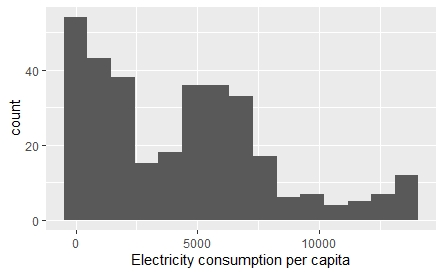
\includegraphics[scale=.65]{electricidad_antes.jpeg}}
\caption{Histograma del consumo per capita de electricidad sin corregir}
\label{fig}
\end{figure}\\



\begin{figure}[htbp]
\centerline{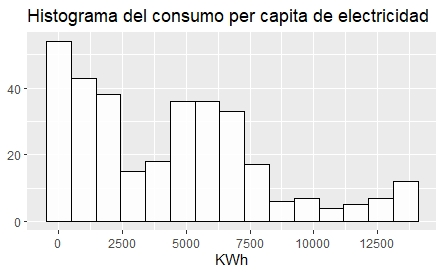
\includegraphics[scale=.60]{electricidad.jpeg}}
\caption{Histograma del consumo per capita de electricidad corregida}
\label{fig}
\end{figure}\\



\begin{figure}[htbp]
\centerline{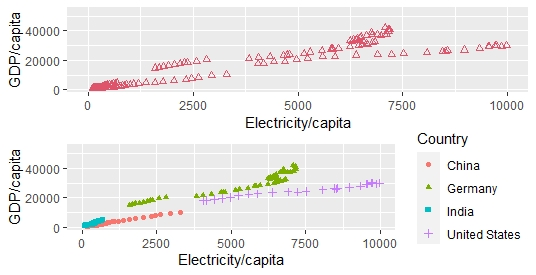
\includegraphics[scale=.60]{PBI_y_Elec_antes.jpeg}}
\caption{GDP y el consumo de electricidad per cápitas sin corregir}
\label{fig}
\end{figure}\\



\begin{figure}[htbp]
\centerline{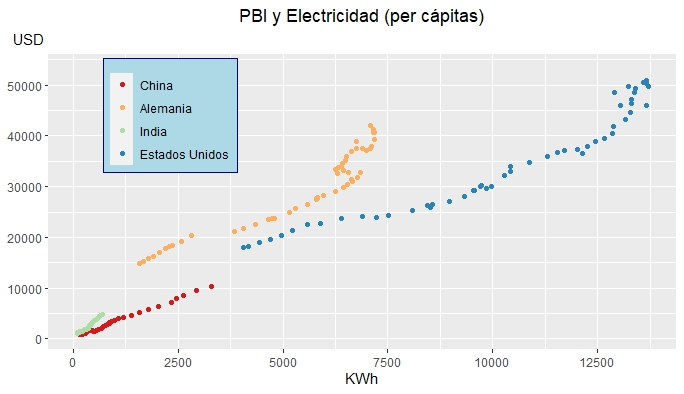
\includegraphics[scale=.60]{PBI_y_Elec.jpeg}}
\caption{GDP y el consumo de electricidad per cápitas corregidos}
\label{fig}
\end{figure}\\




\begin{figure}[htbp]
\centerline{\includegraphics[scale=.65]{reg_pbi_elec_antes.jpeg}}
\caption{Regresión PBI  y electricidad per cápita sin corregir}
\label{fig}
\end{figure}\\



\begin{figure}[htbp]
\centerline{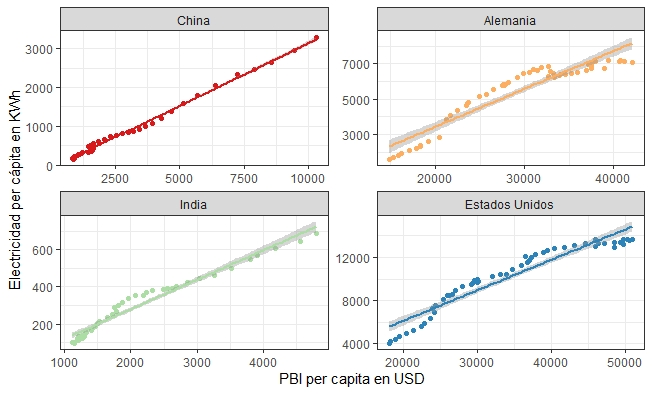
\includegraphics[scale=.65]{reg_pbi_elec_sin.na.jpeg}}
\caption{Regresión PBI  y electricidad per cápita corregido}
\label{fig}
\end{figure}\\











\maketitle









\end{document}
